Dieser Versuch befasst sich mit der Messung der Wirk- und Blindleistung mithilfe eines Multiplikators und eines trägen Messgerätes. Es wird zusätzlich die Scheinleistung berechnet, und die berechneten und gemessenen Ergebnisse werden miteinander verglichen.

\subsubsection{Versuchsaufbau}

Der Versuchsaufbau ähnelt weitestgehend dem in Abschnitt \ref{sec:Aufbau2.2.1} beschriebenen. Es wird jedoch das Oszilloskop durch einen Multiplikator und ein träges, analoges Messgerät gemäß Abbildung \ref{fig:Plan2-2} ersetzt. Das Messgerät wird auf Gleichspannung eingestellt und misst somit den Gleichanteil der Spannung $u_P(t)$, welche durch die Multiplikation von Spannung $u_U(t)$ und zum Strom proportionalen Spannung $u_I(t)$ eine zur Momentanleistung proportionale Größe dar stellt. Somit kann nach Bestimmung des Proportionalitätsfaktors die Wirkleistung gemessen werden.

\begin{figure}[H]
\centering
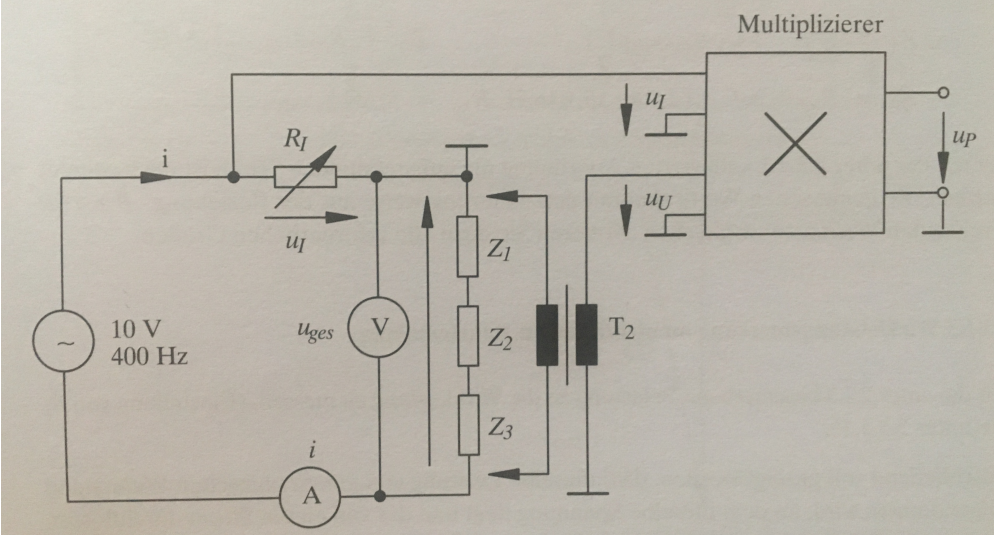
\includegraphics[width=0.7\linewidth]{Images/Aufbau2-2.png}
\caption{Schaltplan eines Versuches zur Messung der Wirkleistung eines Schaltkreises}
\label{fig:Plan2-2}
\end{figure}
Die Impedanzen $Z_1$ bis $Z_3$ werden je nach zu messender Größe verändert.

\subsubsection{Kalibrierung des Drehspulmessinstrumentes}
Damit die Wirkleistung aus den am Messgerät abgelesenen Werten errechnet werden kann, muss die Proportionalitätskonstante, im Folgenden "K", sowie der Offset des Multiplizierers bestimmt werden.
Es gilt:
\begin{equation}
K\cdot \overline{u_P(t)} = P
\label{eq:PropFaktor}
\end{equation}

Der Offset wird gemessen indem die Anschlüsse des potentialtrennenden Transformators kurzgeschlossen werden. $u_U(t)=0$ gilt nun, d.h. das Messgerät sollte null anzeigen.
Angezeigt wird jedoch ein Wert von $-1mV$, d.h. die gemessenen Werte müssen um $1mV$ korrigiert werden. Alle im Folgenden aufgeführten Messwerte wurden um diesen Faktor bereits korrigiert.

Es wird $Z_1 = 40\Omega; Z_2 = Z_3 = 0\Omega$ eingebaut. $u_{ges}$ wird durch Veränderung von $R_I$ auf 6V eingestellt. $I_{ges}$ wird hierbei als $0.16A$ gemessen. Durch eine Phasenverschiebung von $\varphi = 0$ am ohm'schen Verbraucher lässt sich nun die Wirkleistung entsprechend \eqref{eq:LeistungGleichanteil} berechnen als:
\begin{equation*}
P_{mes}=U_{ges}I_{ges} = 6V\cdot 0.16A = 0.96W
\end{equation*}
Das Messgerät zeigt eine Spannung von $\overline{u_P}=0.475V$ an. 
Durch Umstellen von Gleichung \eqref{eq:PropFaktor} lässt sich nun der Proportionalitätsfaktor bestimmen:
\begin{equation*}
K=\frac{P_{mes}}{\overline{u_P}} = \frac{0.96W}{0.475V} = 2.021A
\end{equation*}

\subsubsection{Messung der Wirkleistung}

Dieser Versuchsteil befasst sich mit der Messung der Wirkleistung, welche von verschiedenen Verbrauchern aufgenommen wird. Der Versuchsaufbau gleicht dem vorherigen Versuchsteil, bis auf die Impedanzen. Für sie gilt nun:
\begin{itemize}
\item $Z_1 = \frac{1}{j\omega C} \mbox{ mit } C = 6\mu F$
\item $Z_2 = [30; 40; \cdots; 80]\Omega$
\item $Z_3 = R_{sp} + j\omega L \mbox{ mit } L = 15,84mH; R_{sp} = 5,5\Omega$
\end{itemize}
$R_I$ darf hierbei nicht mehr verändert werden. Grund dafür ist, dass die Spannung $u_I$, welche zur Berechnung von $u_P$ und somit der Wirkleistung verwendet wird, von $R_I$ abhängt.
Im Folgenden wird $Z_2$ variiert. Die Spannung $\overline{u_P}$ wird abgelesen und mit Gleichung \eqref{eq:PropFaktor} die Wirkleistung berechnet. Zusätzlich werden $U_{ges}$ und $I$ an den Messgeräten abgelesen.

Folgende Messwerte wurden aufgenommen:

\begin{center}
\begin{tabular}{| c | c | c | c | c |}
\hline
$\frac{Z_2}{\Omega}$ & $\frac{\overline{u_P}}{V}$ & $\frac{P_{mes}}{W}$ & $\frac{U_{ges}}{V}$ & $\frac{I_{ges}}{A}$ \\
\hline
\end{tabular}
\end{center}